%
% Annual Cognitive Science Conference
% Sample LaTeX Two-Page Summary -- Proceedings Format
%

% Original : Ashwin Ram (ashwin@cc.gatech.edu)       04/01/1994
% Modified : Johanna Moore (jmoore@cs.pitt.edu)      03/17/1995
% Modified : David Noelle (noelle@ucsd.edu)          03/15/1996
% Modified : Pat Langley (langley@cs.stanford.edu)   01/26/1997
% Latex2e corrections by Ramin Charles Nakisa        01/28/1997
% Modified : Tina Eliassi-Rad (eliassi@cs.wisc.edu)  01/31/1998
% Modified : Trisha Yannuzzi (trisha@ircs.upenn.edu) 12/28/1999 (in process)
% Modified : Mary Ellen Foster (M.E.Foster@ed.ac.uk) 12/11/2000
% Modified : Ken Forbus                              01/23/2004
% Modified : Eli M. Silk (esilk@pitt.edu)            05/24/2005
% Modified : Niels Taatgen (taatgen@cmu.edu)         10/24/2006
% Modified : David Noelle (dnoelle@ucmerced.edu)     11/19/2014

%% Change "letterpaper" in the following line to "a4paper" if you must.

\documentclass[10pt,letterpaper]{article}

\usepackage{cogsci}
\usepackage{pslatex}
\usepackage{apacite}
\usepackage{graphicx}



\title{Tutorial: Meta-Analytic Methods for Cognitive Science}

\author{{\large \bf Sho Tsuji } \\
    \texttt{tsujish@gmail.com}\\
  D\'epartement d'Etudes Cognitives\\
   Ecole Normale Sup\'erieure
  \And {\large \bf Molly Lewis} \\
  \texttt{mll@stanford.edu}\\
    Department of Psychology\\
    Stanford University
  \And {\large \bf Mika Braginsky} \\
    \texttt{mikabr@stanford.edu}\\
      Department of Psychology\\
      Stanford University
  \AND {\large \bf Christina Bergmann} \\
      \texttt{chbergma@gmail.com}\\
  D\'epartement d'Etudes Cognitives\\
   Ecole Normale Sup\'erieure
     \And      {\large \bf Page Piccinini } \\
     \texttt{page.piccinini@gmail.com}\\
  D\'epartement d'Etudes Cognitives\\
   Ecole Normale Sup\'erieure
  \And        {\large \bf Michael C. Frank} \\
     \texttt{mcfrank@stanford.edu}\\
            Department of Psychology \\
            Stanford University
  \AND          {\large \bf Alejandrina Cristia} \\
      \texttt{alecristia@gmail.com}\\
  D\'epartement d'Etudes Cognitives\\
   Ecole Normale Sup\'erieure}

\begin{document}

\maketitle

\begin{quote}
\small
Meta-analysis is a powerful and underused tool in cognitive science. It allows researchers to leverage entire bodies of literature to get a broad and quantitative overview of a particular phenomenon, thereby promoting theory development, and to make more precise estimates of effect sizes, which enables robust planning of prospective studies (e.g. through power-analyses). In this tutorial, we will introduce meta-analysis as an analytical tool, and provide participants with hands-on experience conducting their own meta-analysis. We will also present an online platform we have developed for conducting meta-analyses in the field of language development: MetaLab (\url{http://metalab.stanford.edu}). 

\textbf{Keywords:}
meta-analysis; reproducability
\end{quote}


% Tutorials allow participants to gain new insights, knowledge, and skills from a broad range of topics in the field of cognitive science. Tutorials must cover a well-established topic or method, and should be delivered by one or more experts in that area. Tutorials should be presented at a level that will make the material accessible to a postgraduate student with a first degree in a discipline or area of cognitive science. We strongly encourage an interactive delivery format. Tutorials may either be a half-day or full-day in duration. Half-day tutorials are about 3 hours long (not including breaks). Full-day tutorials are about 6 hours long (not including breaks). Proposals should be submitted as two-page summaries that describe the significance of the topic or method, describe the structure and activities to be included in the tutorial, describe the credentials of the tutorial organizer, and include relevant references. (See "Submission Formats," below.) Comments and evaluations from reviewers will be solicited to aid in making decisions about whether or not to accept a given proposal. Organizers of accepted tutorials will be reimbursed for expenses associated with organizing the tutorial, up to a fixed limit ($600 for each half-day tutorial and $1200 for each full-day tutorial that is delivered). If organizers wish to request reimbursement, they need to submit a budget with their proposal. Budgets cannot include travel, hotel, per diems, food/drink (for the session or the organizers), or printed materials. Budgets may include registration costs for individuals that would not otherwise attend the meeting because of demonstrated hardship. Tutorial participants will be charged an extra fee of $30 on top of the regular conference registration. Tutorial organizers will be given access to the email addresses of the preregistered participants so they can contact them in advance about what equipment or supplies to bring, as well as let them know of any preparations that they should make, prior to the tutorial.

\section{Significance}

The empirical social sciences are in crisis: many subfields are plagued by issues of low reliability and validity of their findings \cite{ioannidis2005most,open2013reproducibility,open2015estimating}. One source of this crisis may be the lack of broad, quantitative overviews of a particular research field, which would provide better estimates of true effect sizes and the influence of moderator variables compared to the outcomes of single, and possibly under-powered studies. Meta-analysis is a powerful tool for addressing this issue by quantitatively aggregating across studies in a particular field. They provide, on the one hand, more precise measures of effect sizes and their variability, allowing researchers to base sample size decisions on power analysis. On the other hand, by providing a framework in which different studies can be compared in a quantitative way, researchers can explore relationships between variables previously not compared in a single study, thereby further developing theories based on a broad overview of a particular phenomenon. As such, meta-analyses allow researchers to design new studies robustly, by enablint to make both practical decisions (such as sample size) and theoretical decisions (such as predictions for particular variables) that are grounded in empirical data.


However, despite these benefits, meta-analysis has not become a prevalent tool in cognitive science. One reason may be that there are high hurdles and few immediate rewards to conducting a meta-analysis. Conducting a meta-analysis is a laborious process, particularly according to common practice where a few people do the work, and with little ready-to-use support tools and educational materials available. In addition, the general benefits of meta-analyses, for instance the possibility of conducting power analyses, are often neither evident nor accessible to individual researchers, and so the incentives for conducting analyses are low. Moreover, there seem to be no clear-cut solutions for common criticisms of meta-analyses like "mixing apples and oranges", the file-drawer problem, or publication bias. Finally, traditional meta-analyses remain static after publication, aging quickly as new results emerge.

The goal of this tutorial is to lower these hurdles and demonstrate the potential rewards for conducting meta-analyses. We will start with a broad introduction to meta-analysis as an analytical tool. Participants will then get hands-on experience conducting a meta-analysis in an interactive session. By the end of the tutorial,  participants  will have a better understanding of the practical and theoretical utility of meta-analysis, as well as working knowledge about how to go about conducting their own meta-analysis in a topic of interest.

Part of the focus of the tutorial will be introducing participants to a tool we have been developing for meta-analysis, MetaLab \cite<\url{http://metalab.stanford.edu};>{bergmann2015,lewis2015}. MetaLab is an online platform that aggregates meta-analyses on topics related to language development \cite<e.g., phoneme discrimination and word segmentation;> {tsuji2014perceptual,bergmann2015development}. MetaLab addresses three key challenges in conducting meta-analyses. First, it supplies templates and analysis scripts, streamlining the process of learning about and conducting a meta-analysis. Second, it supports community-augmented meta-analyses  \cite<CAMA;>{tsuji2014community}, allowing a meta-analysis to be conducted and extended by multiple researchers, both reducing the workload of the individual researcher as well as allowing for dynamic extensions to always include the newest results. Third, for each meta-analysis conducted in the MetaLab framework, we provide free and easy-to-use tools for power analysis and data exploration (Fig. 1).

A broad range of researchers will benefit from this introduction to meta-analysis: Novices to a particular research subfield who are in need of a robust overview can turn their literature review into a meta-analysis with a few additional steps, providing themselves and the whole research community with a valuable resource. Any researcher faced with new requirements for publishing in top-tier journals, such as providing a reason for sample size decisions, will profit from being familiar with the concept and uses of meta-analyses, including thinking in terms of effect sizes rather than significance. 


\begin{figure}[t]
\begin{center}
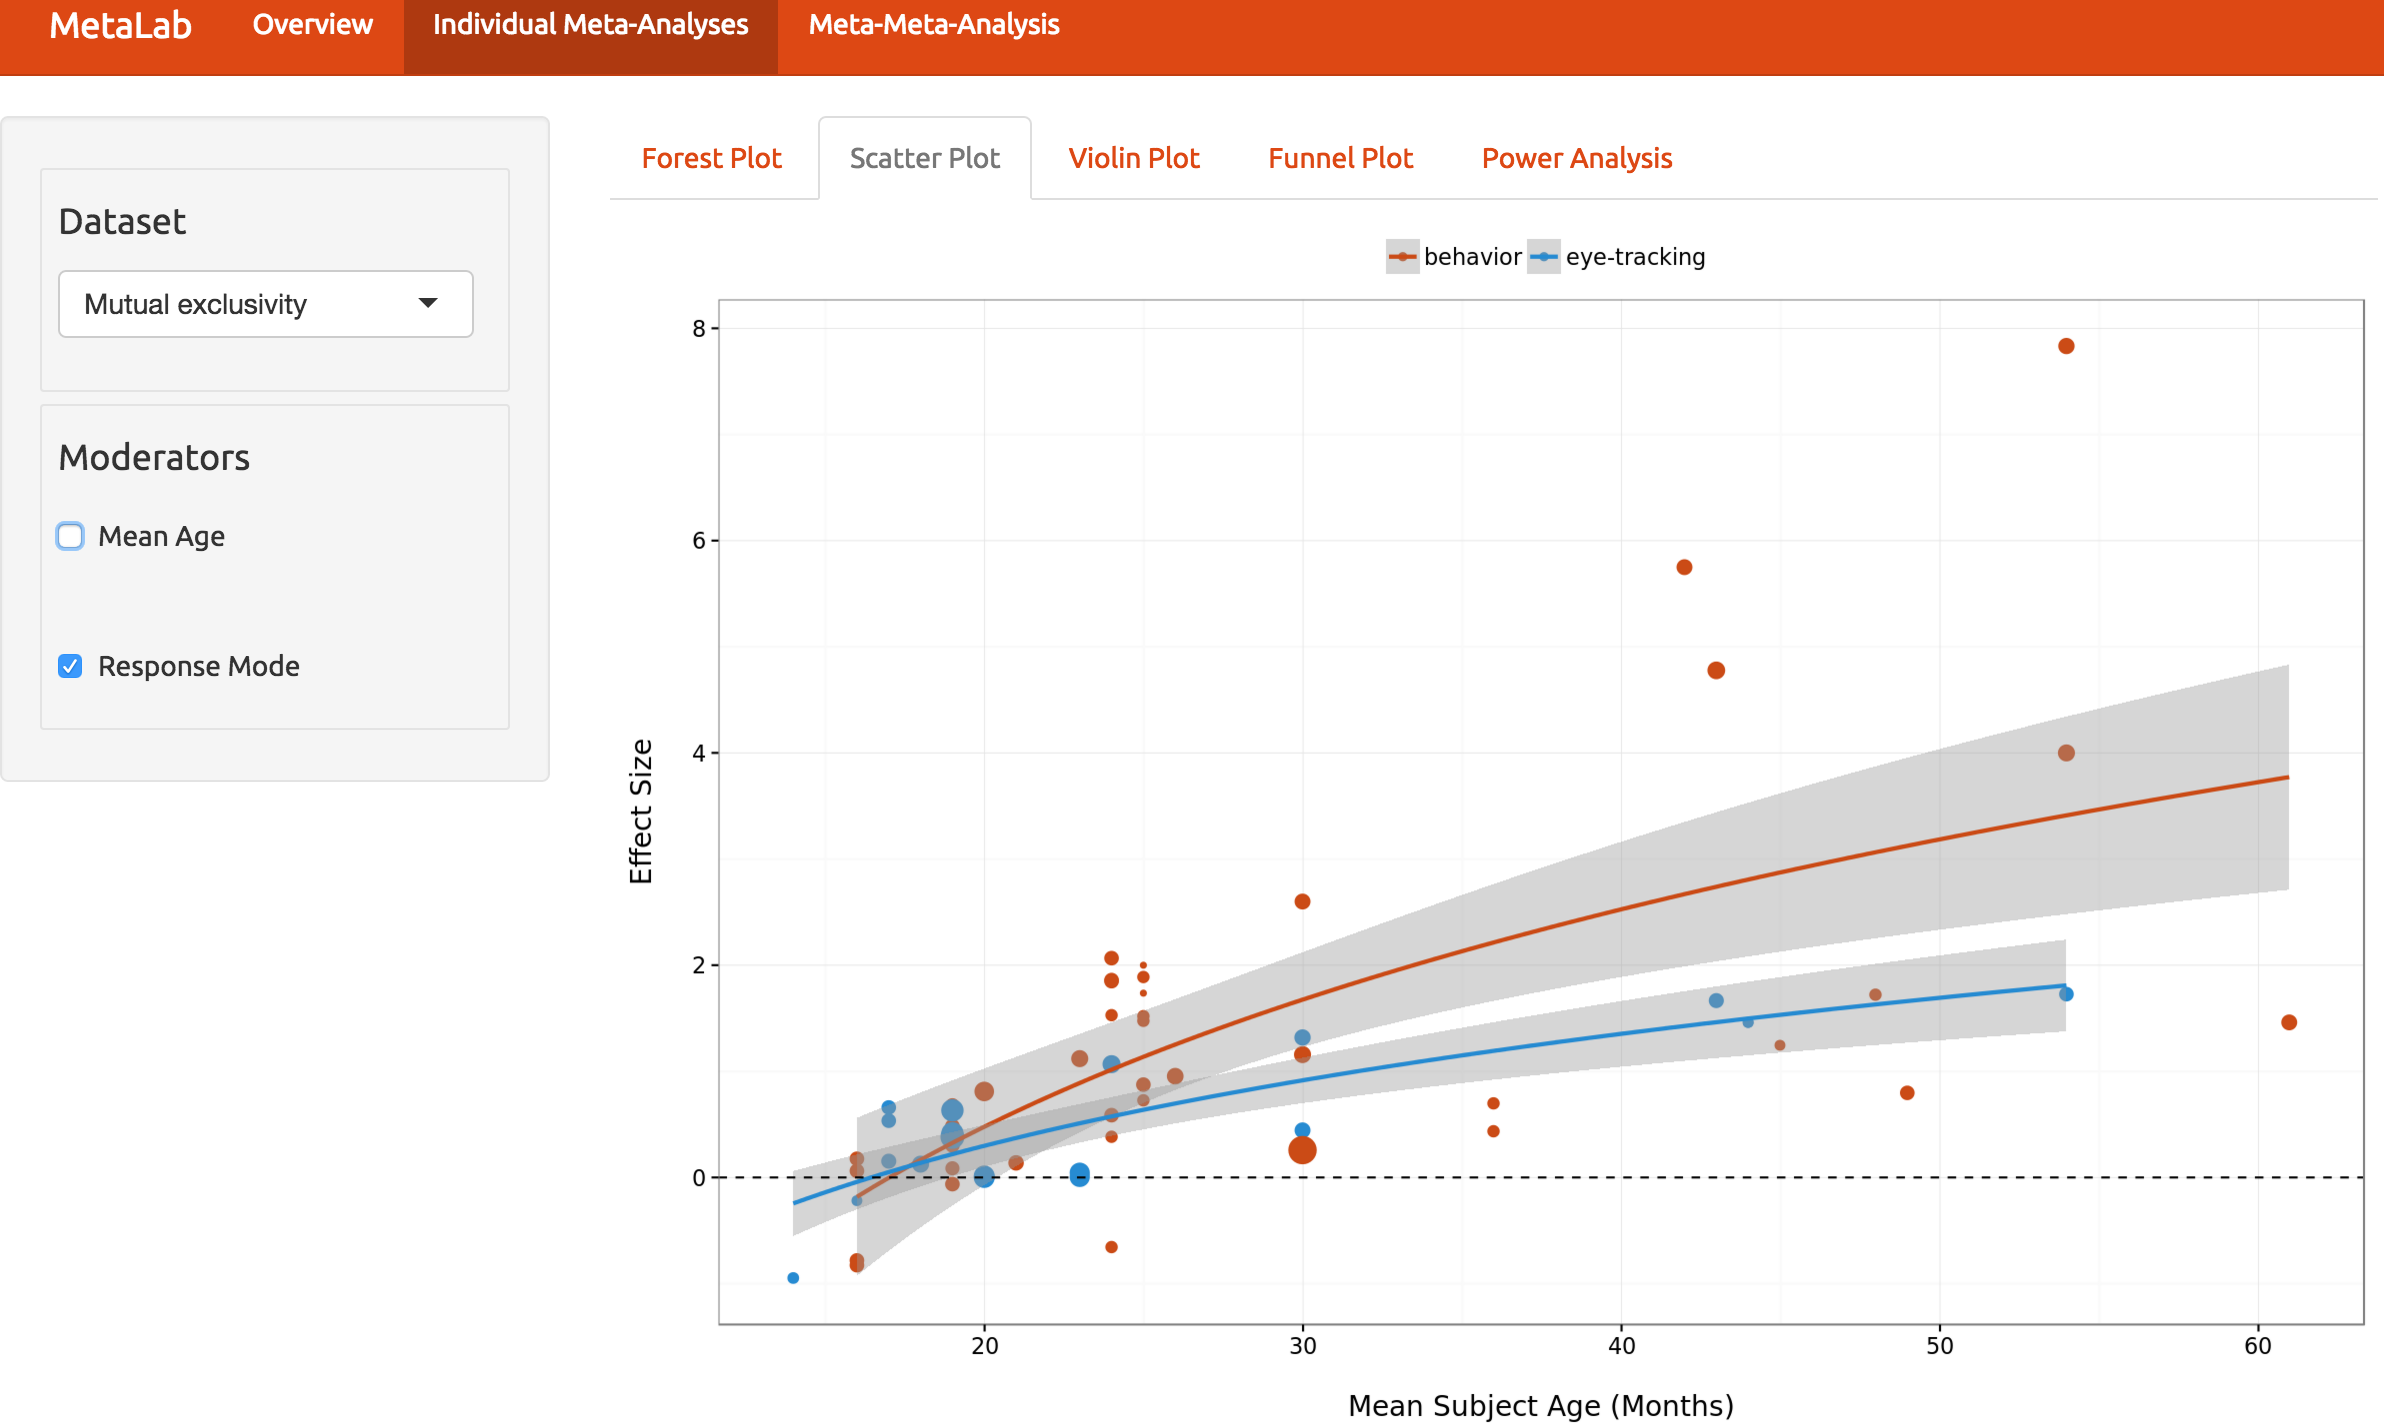
\includegraphics[scale = .2]{power_calculator2.png}
\end{center}
\vspace{-.5em}
\caption{Screenshot of the MetaLab interactive tool. For each meta-analysis in the database, MetaLab provides a set of visualization tools, allowing users to interactively explore the role of moderators on effect sizes. Here, we see an increase in effect size for the bias to select a novel referent for a novel word (mutual exclusivity) across development, and as a function of method. }
\label{fig:lev}
\vspace{-1em}
\end{figure}

\section{Structure}

This one-day tutorial will introduce participants to the method of meta-analysis, providing a hands-on step-by-step guide to use the MetaLab infrastructure for conducting a meta-analysis, working on it collaboratively, and sharing it with the research community.

We will lead participants through the steps of a meta-analysis based on a pre-selected topic. The topics of literature search and study selection, which precede the actual meta-analysis, will be covered briefly, but not  be included in the hands-on part of the tutorial. Participants will be walked through the steps of a meta-analysis with a theoretical and practical component to each step of the process. Two tutorial organizers will be available for questions and assistance throughout the tutorial.

\begin{enumerate}
    \item Coding of variables (2h)
    \begin{enumerate}
        \item Theory: How to decide on independent and dependent variables to be included; which information is needed
        \item Practical: Set-up of a spreadsheet in standardized format, deciding on variables to be included, coding of one pre-selected article (different article for each participant)
    \end{enumerate}
    \item Effect size calculation (1h)
    \begin{enumerate}
        \item Theory: Introduction to different types of effect sizes, their calculation, and how to transform between them
        \item Practical: Effect size calculation for paper coded
    \end{enumerate}
    \item Meta-analysis (3h)
    \begin{enumerate}
        \item Theory: Introduction to meta-analytic regression, choice of model, choice of moderator variables, correction for publication bias, and interpretation of analysis output
       \item Practical: Putting together the papers coded by each participant and conducting a meta-analysis
        \end{enumerate}
\end{enumerate}

Each participant will need a laptop, but no additional materials are required for the tutorial.


\section{Organizer Credentials}
 All organizers have conducted meta-analyses in their field. We have also worked together to develop the MetaLab platform since 2/2015. AC, CB, and ST have expertise creating CAMAs \cite{tsuji2014community}. ST, ML, CB, and AC have experience leading meta-analysis workshops. MB, MF, ML, and PP have experience with web development, dynamic data entry, and online statistical analyses. ST and ML will be present for the tutorial. 


\bibliographystyle{apacite}

\setlength{\bibleftmargin}{.125in}
\setlength{\bibindent}{-\bibleftmargin}

\bibliography{metalab_tutorial}
\end{document}
